\subsection{CLM-Stabilitätskriterium}
\begin{tcolorbox}[colback=white!10!white,
                  colframe=green!30!black,
                  title=CLM-Kriterium] 
    \textbf{Annahme:}
    $m$-Wurzeln in RHE  und $n-m$-Wurzeln ($n \leq m$)
    
    Charakteristische Gleichung:
    \begin{align*}
        P(s) = a_0 + a_1s + a_2s^2 + \ldots + a_n s^n = 0 
    \end{align*}
    Einsetzen $s = j\omega$.
    Das System ist dann asymptotisch stabil, wenn
    \begin{enumerate}
        \item die Ortskurve $P(j\omega)$  für $0 \leq \omega \leq \infty$ die 
            Quadranten abwechselnd durchläuft (sich die Nullstellen des Real- 
            und Imaginärteils von $P(j\omega) = U(\omega)+iV(\omega)$ 
            abwechseln).
        \item Real- und Imaginärteil zusammen $n$ (Grad der Gleichung) reelle 
            Nullstellen im Bereich $0 \leq \omega \leq \infty$ besitzen.
    \end{enumerate}
    
    \tcblower
    
    \textbf{Beispiel:}
    \begin{align*}
        &P(s) = 2 + 5s +7s^2 +8s^3 +4s^4 +s^5\\
        &P(j\omega) = 2 + 5j\omega + 7(j\omega)^2 +8 (j\omega)^3 + 4 (j\omega)^4 + (j\omega)^5\\
        &2-7\omega^2 +4\omega^4 + j (5\omega - 8\omega^3 +\omega^5)\\
        &U(\omega) + jV(\omega)
    \end{align*}
    Realteil hat die Nullstellen:
    \begin{align*}
        &2-7\omega^2 +4\omega^4 = 0 \\
        &\omega_1^2 = 0,36 & \omega_2^2= 1,39
    \end{align*}
    Imaginärteil hat die Nullstellen:
        \begin{align*}
            &5\omega - 8\omega^3 +\omega^5= 0 \\
            &\omega_3 = 0  & \omega_4^2= 0,68 & & \omega_5^2= 7,32 
        \end{align*}
    Insgesamt sind $n=5$ reelle Nullstellen mit $\omega_i >= 0$ vorhanden. 
    Diese wechseln sich jeweils ab, damit ist das System asymptotisch stabil. 
    $\omega_3 < \omega_1 < \omega_4 < \omega_2 < \omega_5$ Siehe Grafik:
    \begin{figure}[H]
        \centering
        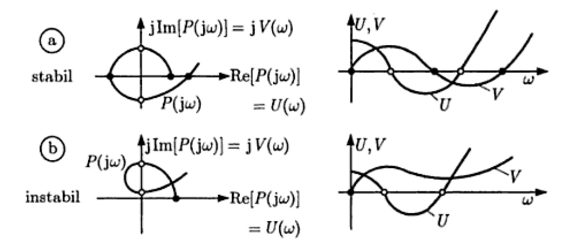
\includegraphics[width=0.7\linewidth]{images/clm}
        \label{fig:clm}
    \end{figure}
\end{tcolorbox}
